\documentclass[10pt]{article}

\usepackage[margin=0.82in]{geometry}
\usepackage{amsmath}
\usepackage{booktabs}
\usepackage{caption}
\usepackage{subcaption}
\usepackage{float}
\usepackage{fontspec}
\usepackage{graphicx}
\usepackage{hyperref}
\usepackage[numbers,sort&compress]{natbib}
\usepackage{placeins}

\newfontfamily\symbolfont{DejaVu Sans}
\newcommand{\taskface}{\raisebox{0pt}[1.2ex][0.2ex]{{\symbolfont\scriptsize ⌐ ͡■ ͜ʖ ͡■}}}
\newcommand{\tasktitle}{Eye-Tracking-Based Reading Time Prediction (\taskface)}

\graphicspath{{figures/}{./}}

\title{
  \vspace{-2.0em}
  
\includegraphics[height=1.25cm]{logo.png}\\[0.6em]
  Nitro NLP Hackathon 5th Edition Submission Writeup\\
  \large \tasktitle
}
\author{\normalsize\bfseries Răzvan-Matei Dedu \hspace{0.35em} Tudor Morariu \hspace{0.35em} Mihnea-Teodor Stoica \hspace{0.35em} David Ștefan Tache}
\date{}

\begin{document}
\maketitle

\section*{Summary}

This is our submission writeup for the Nitro NLP Hackathon 5th Edition. Nitro describes the hackathon as a 23-hour NLP competition for high-school and bachelor students, organized by the Nitro Association, where teams receive a fresh NLP dataset and build leaderboard-scored models under a short deadline \citep{nitrohackathon2026}.

The task, \emph{Eye-Tracking-Based Reading Time Prediction} (\taskface), was to predict Romanian word-level Total Reading Time (TRT), measured from eye-tracking data. Our final solution is a compact tabular model with three main ingredients: word-level target aggregation, rich hand-built lexical and positional features, and frozen Romanian BERT contextual embeddings compressed with PCA. A LightGBM regressor trained on square-root transformed TRT produced a local mean word-level CV score of \textbf{87.19} and a row-level out-of-fold score of \textbf{44.46}.

\section{Task and Data}

Each training row contains a word occurrence, participant id, text id, and observed TRT in milliseconds. The test set contains the same word/text identifiers and a \texttt{datapointID}, but no target. The official submission is a CSV with \texttt{subtaskID}, \texttt{datapointID}, and \texttt{answer}.

Because train and test \texttt{word\_id}s do not overlap, we model general word difficulty rather than memorizing word ids. We aggregate training labels by \texttt{word\_id} using the mean TRT, then map word-level out-of-fold predictions back to the original participant rows for local validation.

\begin{table}[H]
\centering
\caption{Dataset summary used by the final solution.}
\label{tab:data}
\begin{tabular}{lr}
\toprule
Quantity & Value \\
\midrule
Training rows & 135,210 \\
Test rows & 9,425 \\
Training word ids & 4,507 \\
Test word ids & 1,885 \\
Train/test word-id overlap & 0 \\
Training participants & 30 \\
Test participants & 5 \\
Distinct training texts & 9 \\
Row-level zero-rate & 30.62\% \\
Word-level zero-rate after averaging & 0.18\% \\
Mean row-level TRT & 264.44 ms \\
Median row-level TRT & 200.00 ms \\
\bottomrule
\end{tabular}
\end{table}

\begin{figure}[H]
\centering
\begin{subfigure}{0.48\linewidth}
  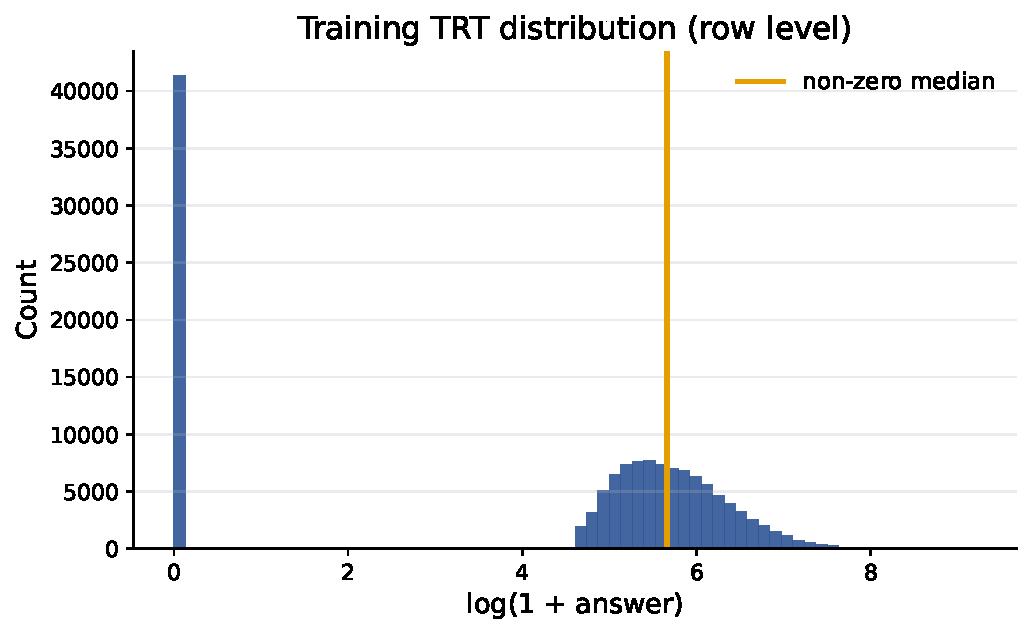
\includegraphics[width=\linewidth]{target_distribution.pdf}
  \caption{Row-level labels}
\end{subfigure}
\hfill
\begin{subfigure}{0.48\linewidth}
  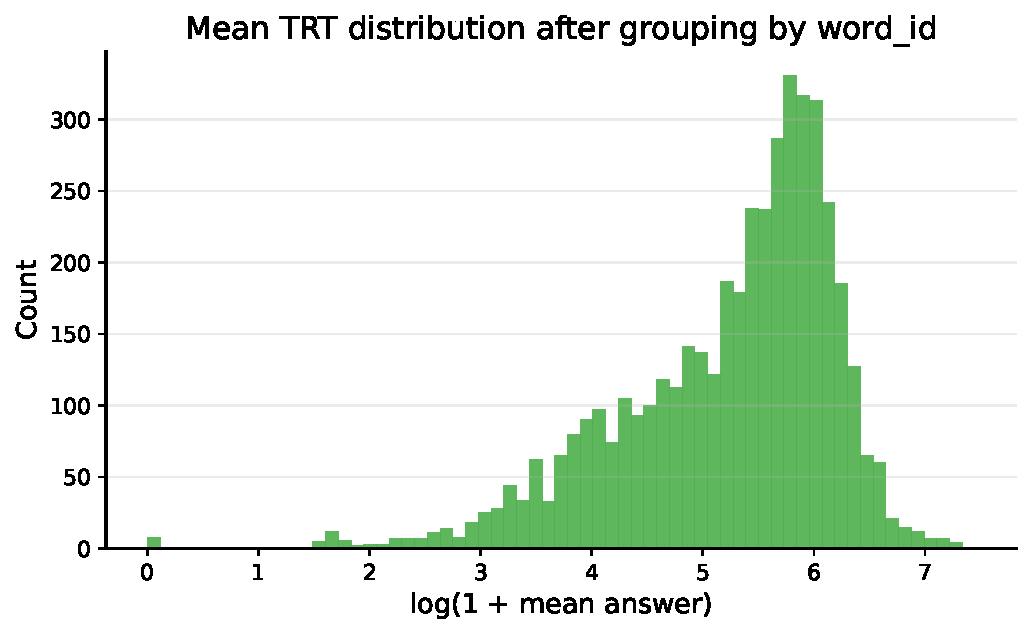
\includegraphics[width=\linewidth]{word_mean_distribution.pdf}
  \caption{Word-level means}
\end{subfigure}
\vspace{0.5em}

\begin{subfigure}{0.56\linewidth}
  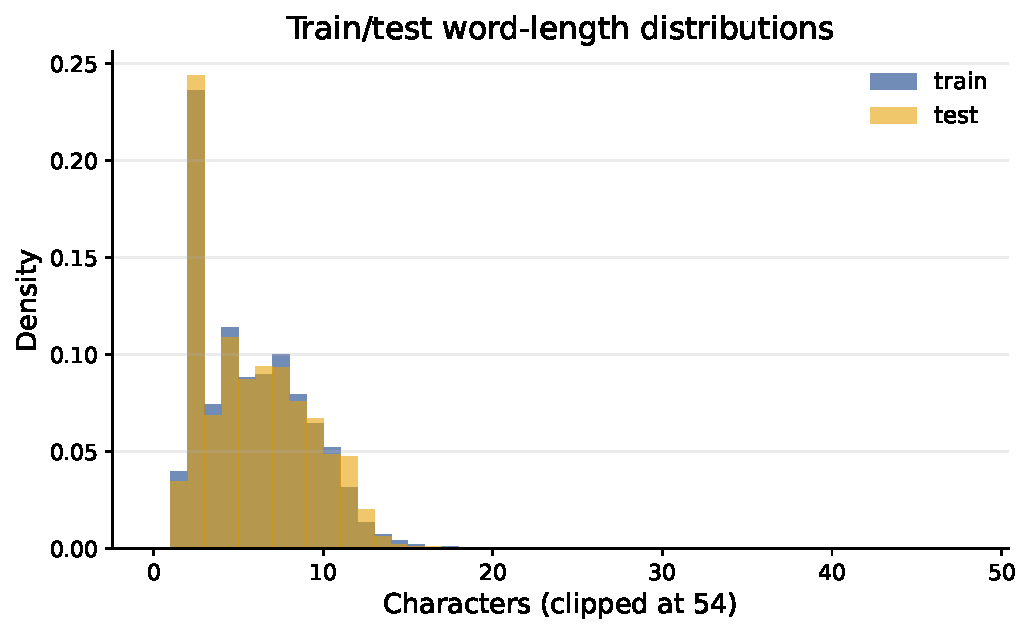
\includegraphics[width=\linewidth]{train_test_length.pdf}
  \caption{Train/test word length}
\end{subfigure}
\caption{Basic data checks. Raw row-level TRT has many zeros; grouping by \texttt{word\_id} gives a smoother target.}
\label{fig:data}
\end{figure}
\FloatBarrier

\section{Evaluation Metric}

The task metric averages non-negative $R^2$ and absolute Pearson correlation:
\begin{equation}
  S(y,\hat y) =
  100 \cdot \frac{\max(0, R^2(y,\hat y)) + |\rho(y,\hat y)|}{2}.
\end{equation}

This metric rewards both calibration and ranking. A model can benefit from getting the relative difficulty of words right, but very large magnitude errors still hurt through the $R^2$ term.

\section{Final Pipeline}

Our final system is deliberately simple to run once embeddings are cached:

\begin{enumerate}
  \item Read \texttt{train\_data.csv}, \texttt{test\_data.csv}, and \texttt{sample\_output.csv}.
  \item Aggregate training labels by \texttt{word\_id}.
  \item Merge auxiliary Romanian eye-tracking and property CSVs from the public eye-tracking repository \citep{ana0101eyetracking}.
  \item Build lexical, position, neighborhood, and categorical word-shape features.
  \item Reconstruct sentence-like contexts and embed each target word with Romanian BERT \citep{dumitrescu2020birth,devlin2019bert}.
  \item Reduce contextual embeddings to 128 PCA components \citep{jolliffe2002pca,pedregosa2011scikit}.
  \item Train repeated stratified LightGBM folds \citep{ke2017lightgbm}.
  \item Average fold predictions and write \texttt{output.csv}.
\end{enumerate}

The implementation is provided in both \texttt{main.ipynb} and \texttt{main.py}. The notebook is a flat procedural version of the solution, matching the way we iterated during the hackathon.

\section{Features}

\textbf{Lexical and shape features.}
We use length, capitalization, punctuation, vowel/consonant counts, syllables, frequency, affixes, and word-shape variants.

\textbf{Position features.}
The \texttt{word\_id} encodes page and within-page position. We derive page index, absolute position, relative page position, distance to page boundaries, and first/last indicators.

\textbf{Local context features.}
For core scalar variables we add previous/next one-word and two-word values plus centered three-word rolling means. These features approximate short-range lexical context without needing a sequence model at training time.

\begin{figure}[H]
\centering
\begin{subfigure}{0.52\linewidth}
  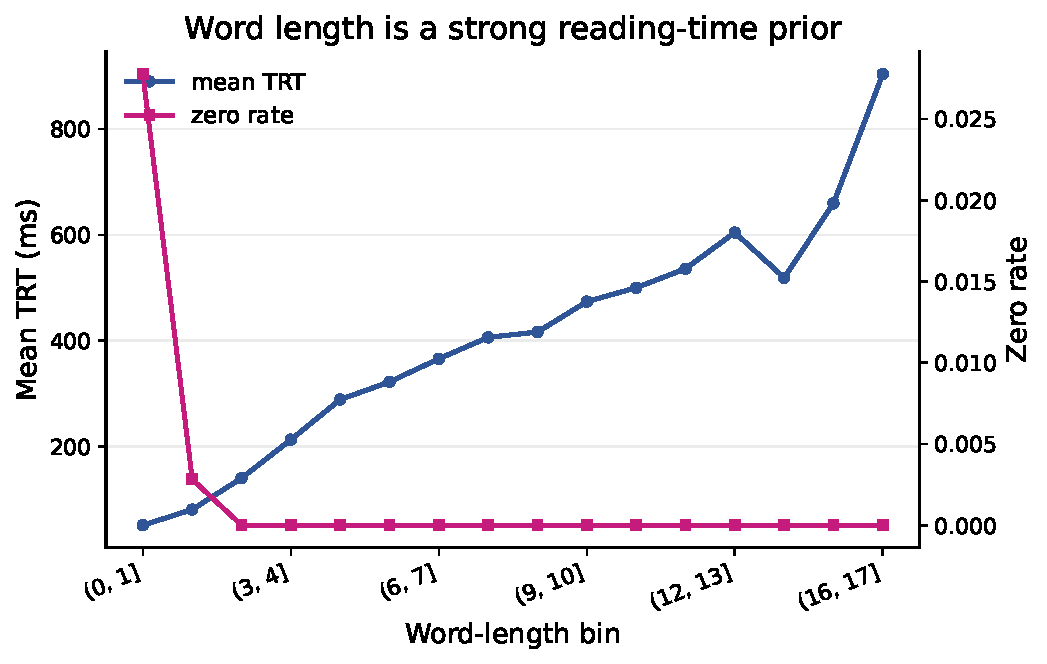
\includegraphics[width=\linewidth]{word_length_effect.pdf}
  \caption{Length prior}
\end{subfigure}
\hfill
\begin{subfigure}{0.44\linewidth}
  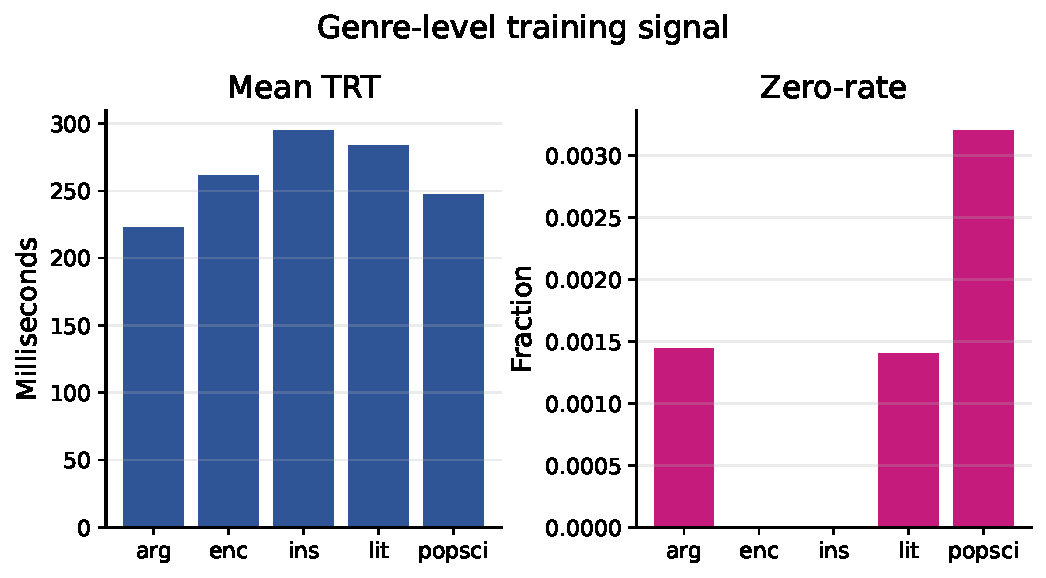
\includegraphics[width=\linewidth]{genre_signal.pdf}
  \caption{Genre signal}
\end{subfigure}
\vspace{0.5em}

\begin{subfigure}{0.56\linewidth}
  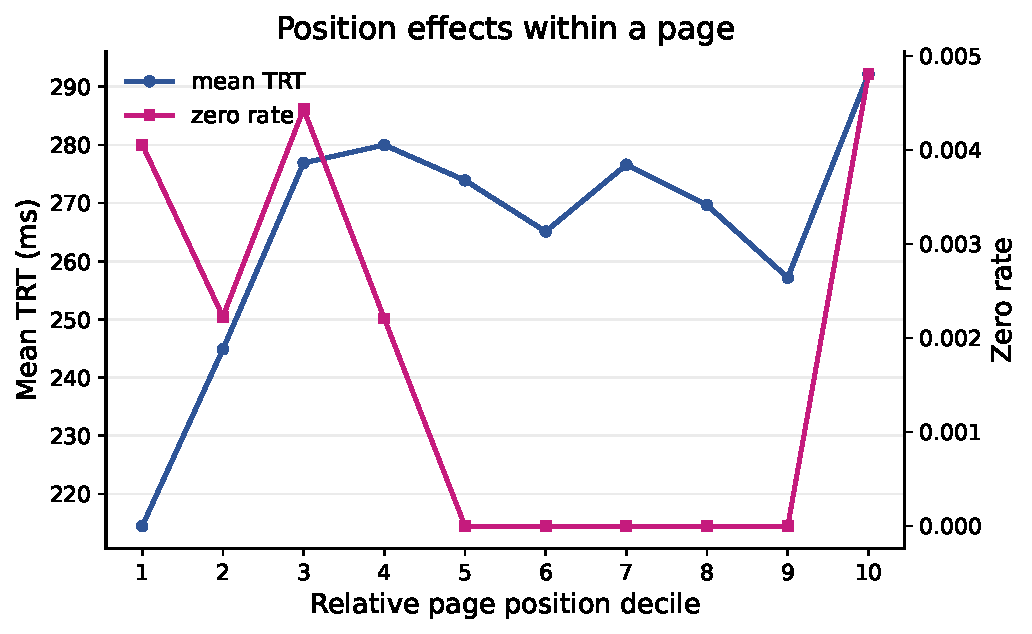
\includegraphics[width=\linewidth]{page_position_trend.pdf}
  \caption{Page position}
\end{subfigure}
\caption{Hand-built features capture meaningful structure before adding neural embeddings.}
\label{fig:features}
\end{figure}

\textbf{Auxiliary eye-tracking features.}
We use Romanian fixation dictionaries and property files from the auxiliary eye-tracking data \citep{ana0101eyetracking,hodivoianu2025predicting,multipleye}. The most useful fields are external TRT summaries, positive-fixation rates, sentence-position information, surprisal, token count, and frequency. For numeric auxiliary columns we add raw, log, square-root, and missingness versions.

\begin{figure}[H]
\centering
\begin{subfigure}{0.44\linewidth}
  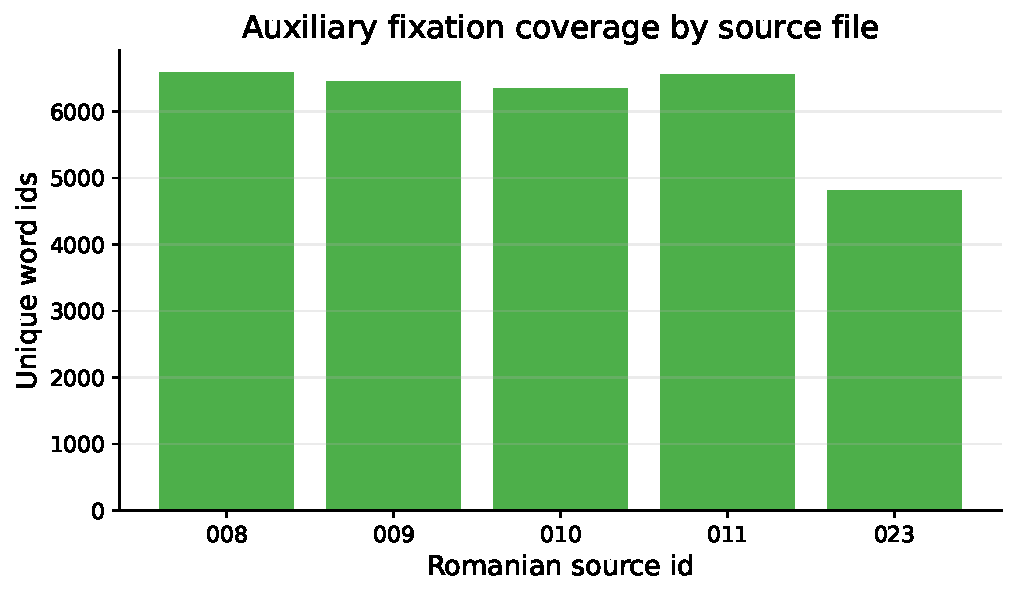
\includegraphics[width=\linewidth]{aux_coverage.pdf}
  \caption{Auxiliary coverage}
\end{subfigure}
\hfill
\begin{subfigure}{0.48\linewidth}
  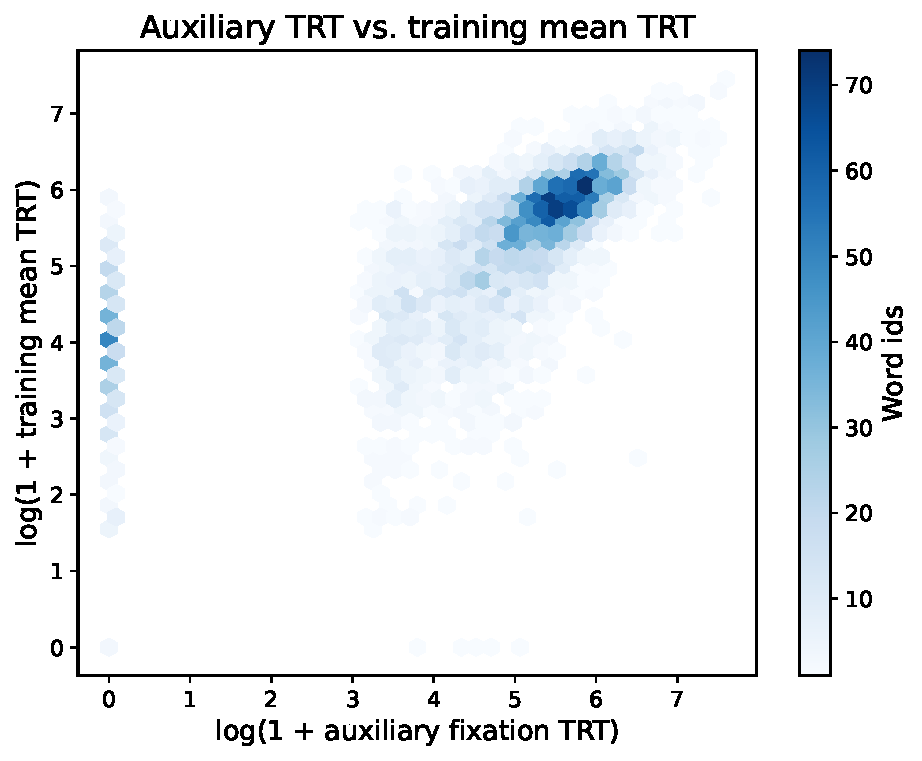
\includegraphics[width=\linewidth]{aux_vs_train.pdf}
  \caption{Auxiliary vs. target}
\end{subfigure}
\vspace{0.5em}

\begin{subfigure}{0.48\linewidth}
  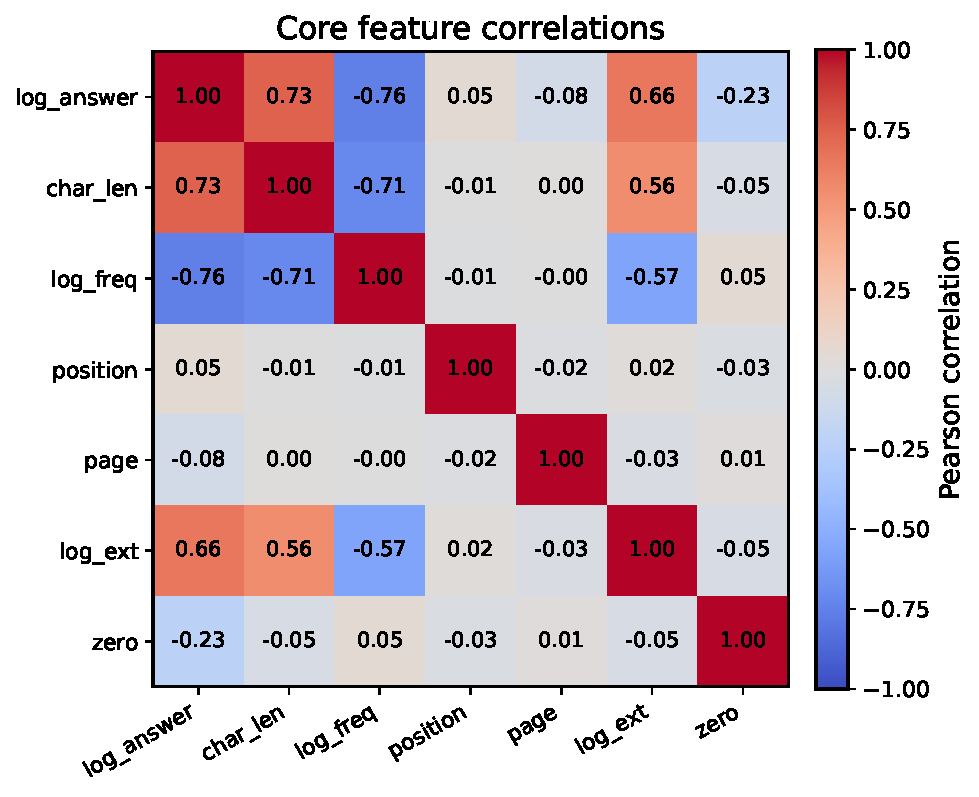
\includegraphics[width=\linewidth]{feature_correlation.pdf}
  \caption{Core correlations}
\end{subfigure}
\caption{Auxiliary fixation measurements were one of the strongest external signals. The log auxiliary TRT to log training mean TRT correlation is 0.656.}
\label{fig:aux}
\end{figure}

\textbf{Contextual embeddings.}
We sort words by text, section, page, and position, then split contexts at sentence-ending punctuation. For each word, we feed up to 48 words on either side into the Romanian BERT model \path{dumitrescustefan/bert-base-romanian-cased-v1}. The word vector is the mean of the target word's subword hidden states. PCA reduces these embeddings to 128 dimensions; the cached run explained 65.76\% of embedding variance.
\FloatBarrier

\section{Model and Training}

The target is transformed as:
\begin{equation}
  z_i = \sqrt{\max(y_i,0)}, \qquad \hat y_i = \max(\hat z_i,0)^2.
\end{equation}
This makes the regression problem less dominated by very large TRT values while keeping predictions non-negative after inversion.

\begin{table}[H]
\centering
\caption{Final LightGBM configuration.}
\label{tab:model}
\begin{tabular}{lr}
\toprule
Parameter & Value \\
\midrule
Trees & 1000 \\
Learning rate & 0.022 \\
Leaves & 15 \\
Minimum child samples & 20 \\
Subsample & 1.0 \\
Column sample by tree & 0.7 \\
L2 regularization & 35 \\
Target transform & square root \\
Fold scheme & 5 folds $\times$ 2 seeds \\
Fold stratification threshold & 90 ms \\
\bottomrule
\end{tabular}
\end{table}

Categorical features are passed directly to LightGBM: genre, normalized word form, prefixes, suffixes, and shape variables. We run 5 stratified folds with seed 42 and 5 more with seed 123, then average all ten test predictions.

\section{Results}

\begin{table}[H]
\centering
\caption{Local validation and output diagnostics.}
\label{tab:results}
\begin{tabular}{lr}
\toprule
Metric & Value \\
\midrule
Mean word-level CV score & 87.19 \\
Row-level OOF score & 44.46 \\
Row-level OOF RMSE & 256.65 ms \\
OOF prediction mean & 258.87 ms \\
OOF prediction std. & 172.32 ms \\
Submission prediction mean & 254.22 ms \\
Submission prediction median & 249.01 ms \\
Submission prediction std. & 162.16 ms \\
Submission prediction max & 1,133.85 ms \\
\bottomrule
\end{tabular}
\end{table}

The word-level validation score is much higher than the row-level score because each word-level prediction is copied back to multiple participant rows. Participant-specific reading behavior remains noisy, but the model is intended to predict general word difficulty for unseen participant-word rows.

\begin{figure}[H]
\centering
\begin{subfigure}{0.48\linewidth}
  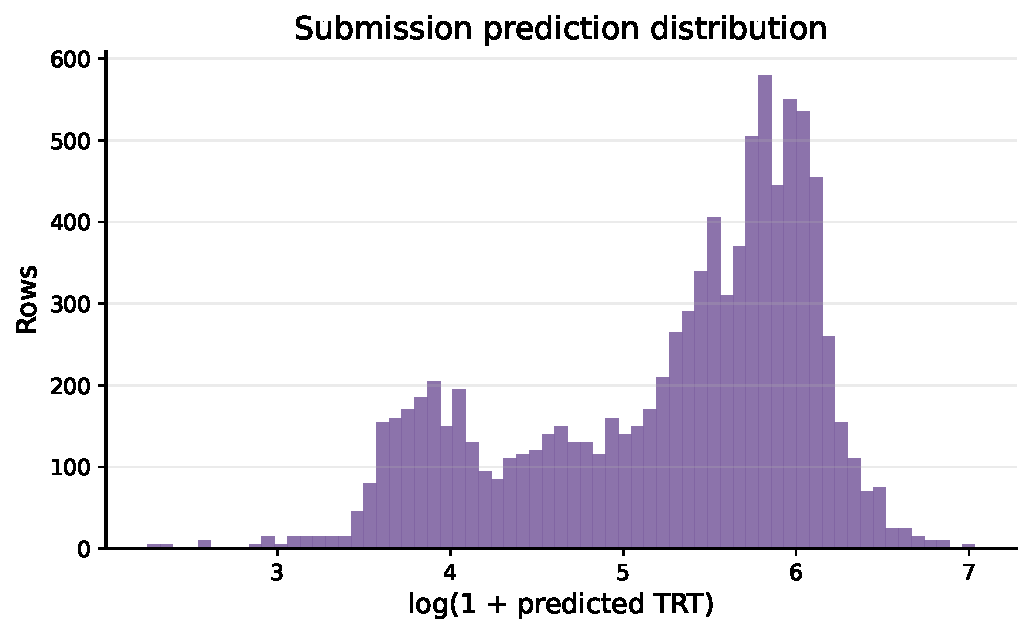
\includegraphics[width=\linewidth]{prediction_distribution.pdf}
  \caption{Prediction distribution}
\end{subfigure}
\hfill
\begin{subfigure}{0.44\linewidth}
  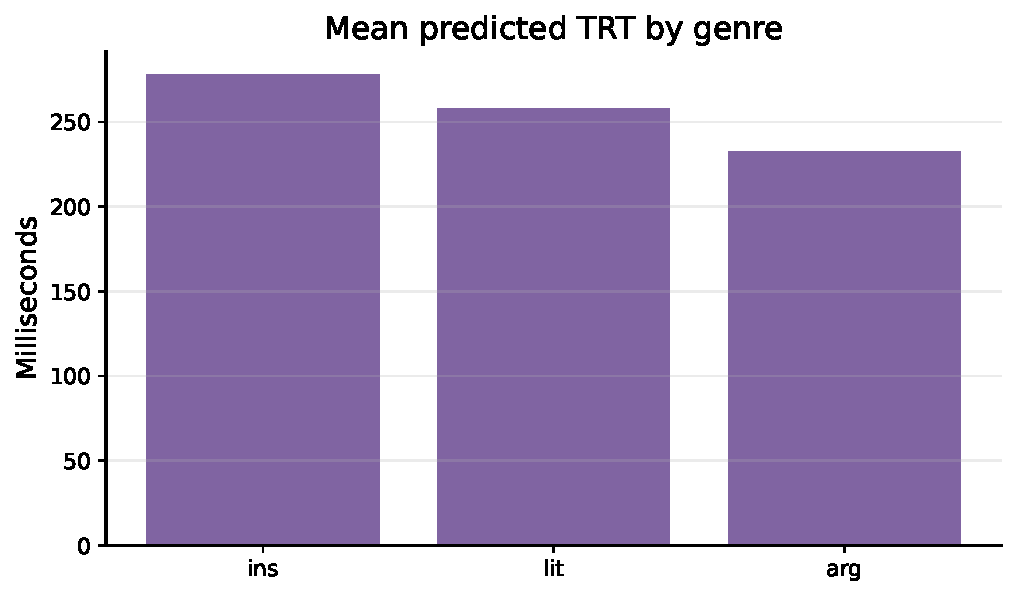
\includegraphics[width=\linewidth]{prediction_by_genre.pdf}
  \caption{Genre means}
\end{subfigure}
\vspace{0.5em}

\begin{subfigure}{0.56\linewidth}
  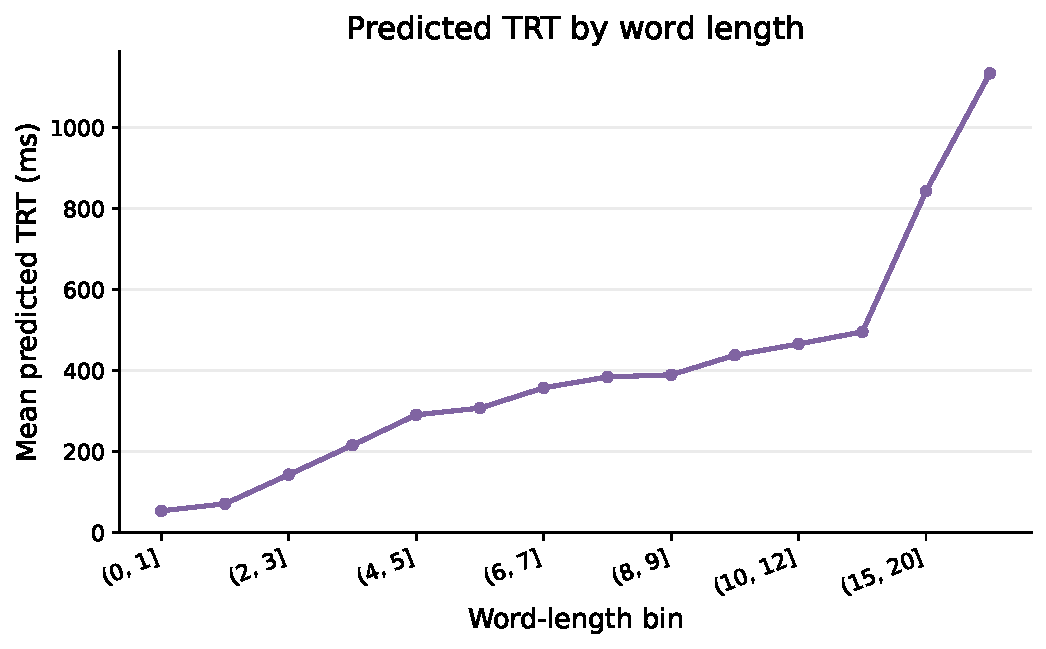
\includegraphics[width=\linewidth]{prediction_length_effect.pdf}
  \caption{Length response}
\end{subfigure}
\caption{Submission diagnostics. Predictions are positive and preserve the expected relationship between word length and reading time.}
\label{fig:predictions}
\end{figure}

\begin{figure}[H]
\centering
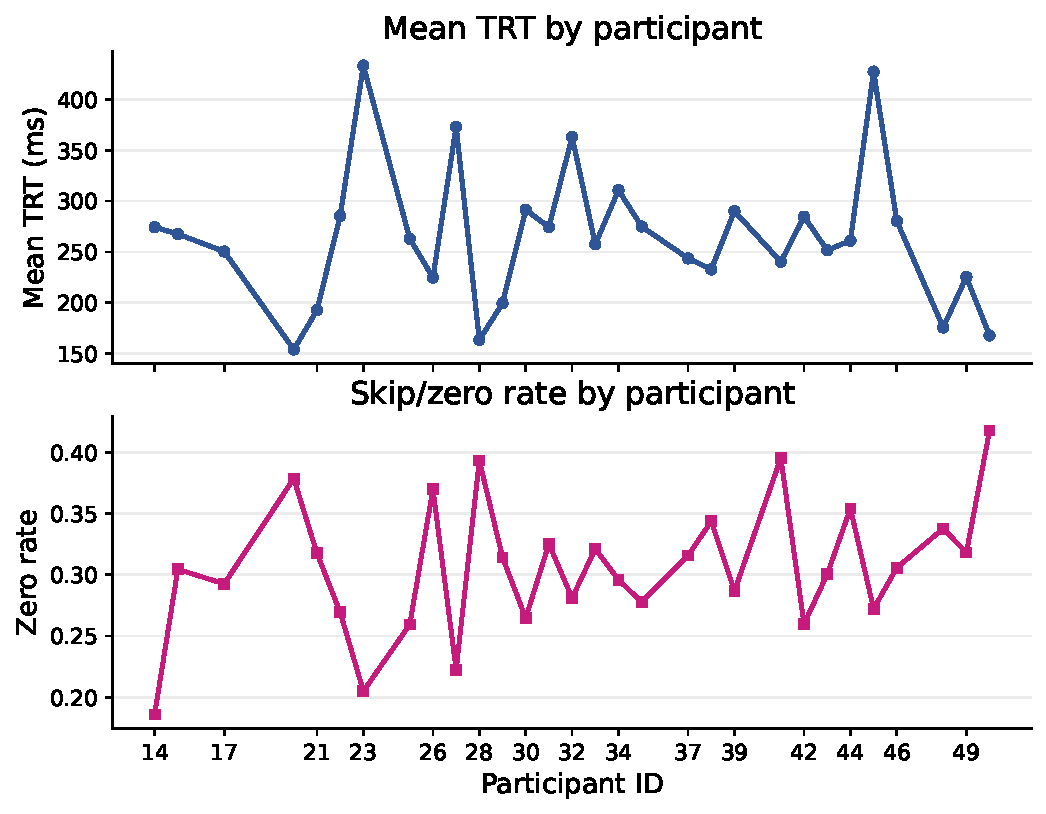
\includegraphics[width=0.74\linewidth]{participant_variation.pdf}
\caption{Participant-level variation in the training data. This motivates aggregating labels by word id.}
\label{fig:participants}
\end{figure}
\FloatBarrier

\section{What Worked}

\begin{itemize}
  \item Aggregating by \texttt{word\_id} made the target substantially cleaner.
  \item Auxiliary fixation files were very valuable because they carried directly related behavioral signal.
  \item Romanian BERT embeddings helped add sentence context without fine-tuning.
  \item The square-root target transform stabilized LightGBM predictions.
  \item Repeated stratified folds reduced variance in the final submission.
\end{itemize}

\section{Limitations}

\begin{itemize}
  \item The model does not explicitly model participant identity at inference time.
  \item PCA is fitted on train and test embeddings together. It uses no labels, but it is still transductive.
  \item The BERT encoder is frozen, so it is not specialized for eye-tracking signals.
  \item Auxiliary files are strong external data; comparisons should state clearly whether they are used.
\end{itemize}

\section{Reproducibility}

The final notebook is \texttt{main.ipynb}. Running it top-to-bottom writes \texttt{output.csv}. The first run may download Romanian BERT weights and build the embedding cache under \texttt{.cache}; later runs reuse the cached embeddings.

Main dependencies are \texttt{numpy}, \texttt{pandas}, \texttt{scipy}, \texttt{scikit-learn}, \texttt{torch}, \texttt{transformers}, \texttt{tqdm}, and \texttt{lightgbm}. Metric and scientific utilities rely on standard Python scientific packages \citep{pedregosa2011scikit,virtanen2020scipy}. ChatGPT was used to help draft and organize this writeup and code presentation \citep{chatgpt2026}.

\clearpage
\bibliographystyle{plainnat}
\bibliography{references}

\end{document}
